\PassOptionsToPackage{dvipsnames}{xcolor}
\documentclass{beamer}

\mode<presentation> {

% The Beamer class comes with a number of default slide themes
% which change the colors and layouts of slides. Below this is a list
% of all the themes, uncomment each in turn to see what they look like.

%\usetheme{default}
%\usetheme{AnnArbor}
%\usetheme{Antibes}
%\usetheme{Bergen}
%\usetheme{Berkeley}
%\usetheme{Berlin}
%\usetheme{Boadilla}
%\usetheme{CambridgeUS}
%\usetheme{Copenhagen}
%\usetheme{Darmstadt}
%\usetheme{Dresden}
%\usetheme{Frankfurt}
%\usetheme{Goettingen}
%\usetheme{Hannover}
%\usetheme{Ilmenau}
%\usetheme{JuanLesPins}
%\usetheme{Luebeck}
%\usetheme{Madrid} % nice one
%\usetheme{Malmoe}
%\usetheme{Marburg}
\usetheme{Montpellier} % good one
%\usetheme{PaloAlto}
%\usetheme{Pittsburgh}
%\usetheme{Rochester}
%\usetheme{Singapore}
%\usetheme{Szeged}
%\usetheme{Warsaw}

% As well as themes, the Beamer class has a number of color themes
% for any slide theme. Uncomment each of these in turn to see how it
% changes the colors of your current slide theme.

%\usecolortheme{albatross}
\usecolortheme{beaver} % I like this one
%\usecolortheme{beetle}
%\usecolortheme{crane}
%\usecolortheme{dolphin}
%\usecolortheme{dove}
%\usecolortheme{fly}
%\usecolortheme{lily}
%\usecolortheme{orchid} % not bad
%\usecolortheme{rose}
%\usecolortheme{seagull}
%\usecolortheme{seahorse}
%\usecolortheme{whale}
%\usecolortheme{wolverine}

%\setbeamertemplate{footline} % To remove the footer line in all slides uncomment this line
\setbeamertemplate{footline}[page number] % To replace the footer line in all slides with a simple slide count uncomment this line

\setbeamertemplate{navigation symbols}{} % To remove the navigation symbols from the bottom of all slides uncomment this line
}

\setbeamertemplate{caption}[numbered]

\usepackage{etex}
\usepackage{array} 
\usepackage{graphicx} % Allows including images
\usepackage{booktabs} % Allows the use of \toprule, \midrule and \bottomrule in tables
\usefonttheme{professionalfonts}
\usepackage{mathptmx}
\usepackage{caption}
\usepackage{subcaption}
\usepackage{amsmath,amsthm,amssymb}
\usepackage{float}
%\usepackage{color}
%\usepackage{tikz}

% ------------------ My own stuff

\usepackage[utf8]{inputenc}
\usepackage[T1]{fontenc}

%\usepackage{hyperref}
%\usepackage{algorithm}
%\usepackage{algpseudocode}
%\usepackage{epigraph}
%\usepackage{caption}
%\usepackage{subcaption}
\usepackage{amsmath,amsthm,amssymb}
\DeclareMathOperator*{\argmax}{\arg\!\max}
\DeclareMathOperator*{\argmin}{\arg\!\min}
\DeclareMathOperator{\E}{\mathbb{E}}
\DeclareMathOperator{\R}{\mathbb{R}}

\beamertemplatenavigationsymbolsempty

\usepackage{rotating}
\usepackage{tikz}

%\usepackage{siunitx}
%\sisetup{group-separator = {,}}

%\usepackage[dvipsnames]{xcolor}
\usepackage{fancyvrb}
\usepackage{listings}
\usepackage{verbatim}

% redefine \VerbatimInput
\RecustomVerbatimCommand{\VerbatimInput}{VerbatimInput}%
{fontsize=\footnotesize,
	%
	frame=lines,  % top and bottom rule only
	framesep=2em, % separation between frame and text
	rulecolor=\color{Gray},
	%
	label=\fbox{\color{Black}Fengyun1Cdebris.tle},
	labelposition=topline,
	%
	commandchars=\|\(\), % escape character and argument delimiters for
	% commands within the verbatim
	commentchar=*        % comment character
}
%----------------------------------------------------------------------------------------
%	TITLE PAGE
%----------------------------------------------------------------------------------------

\title[MEngProject]{Deep Feature Transmission Simulator v2 \\ for \\ Collaborative Intelligence}
\subtitle{TensorFlow 2, Tensor Completion \& Error Concealment} % The short title appears at the bottom of every slide, the full title is only on the title page

\author[Hans]{\large Hans Dhondea \\ {\footnotesize {Supervisor: Prof. Ivan {Bajić}}}} % Your name
\institute[SFU-Multimedia Lab] 
{
Multimedia Lab\\School of Engineering Science\\Simon Fraser University \\ % Your institution for the title page
\medskip
\centering

\includegraphics[scale=0.5]{Figures/SFUhorizontallogorgb.pdf}
}

\date{\today} % Date, can be changed to a custom date

\begin{document}

\begin{frame}
\titlepage % Print the title page as the first slide
\end{frame}

%\addtobeamertemplate{frametitle}{}{%
%\begin{tikzpicture}[remember picture,overlay]
%\node[anchor=south east,yshift=2pt] at (current page.south east)
%{\includegraphics[height=0.9cm]{figs/rrsglogo.pdf}};
%\end{tikzpicture}}

\begin{frame}
\frametitle{Overview} % Table of contents slide, comment this block out to remove it
\tableofcontents % Throughout your presentation, if you choose to use \section{} and \subsection{} commands, these will automatically be printed on this slide as an overview of your presentation
\end{frame}

%%----------------------------------------------------------------------------------------
%%	PRESENTATION SLIDES
%%----------------------------------------------------------------------------------------
\section{Collaborative Intelligence}
\begin{frame}
	\frametitle{Introduction}
	\begin{figure}[H]
		\centering
		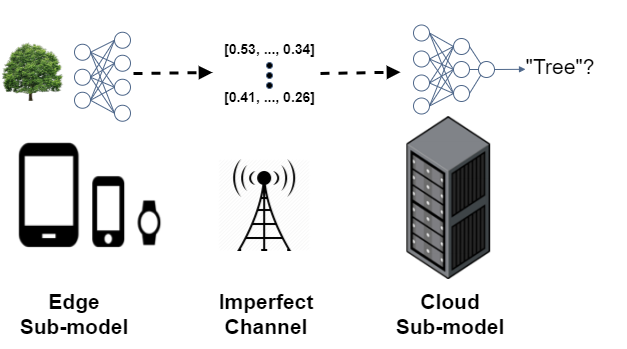
\includegraphics[scale=0.2]{Figures/image--000.png}
		\caption{Blueprint for Collaborative Intelligence.\footnote{\tiny{Y. Kang, J. Hauswald, C. Gao, A. Rovinski, T. Mudge,J. Mars, and L. Tang, “Neurosurgeon: Collaborative intelligence between the cloud and mobile edge,” SIGARCH Comput. Archit. News, vol. 45, p. 615–629, Apr. 2017.}} \cite{neurosurgeon}}
		\label{fig:ci}
	\end{figure}

\end{frame}

\begin{frame}
	\frametitle{Splitting a DNN}
		\begin{figure}[H]
		\centering
		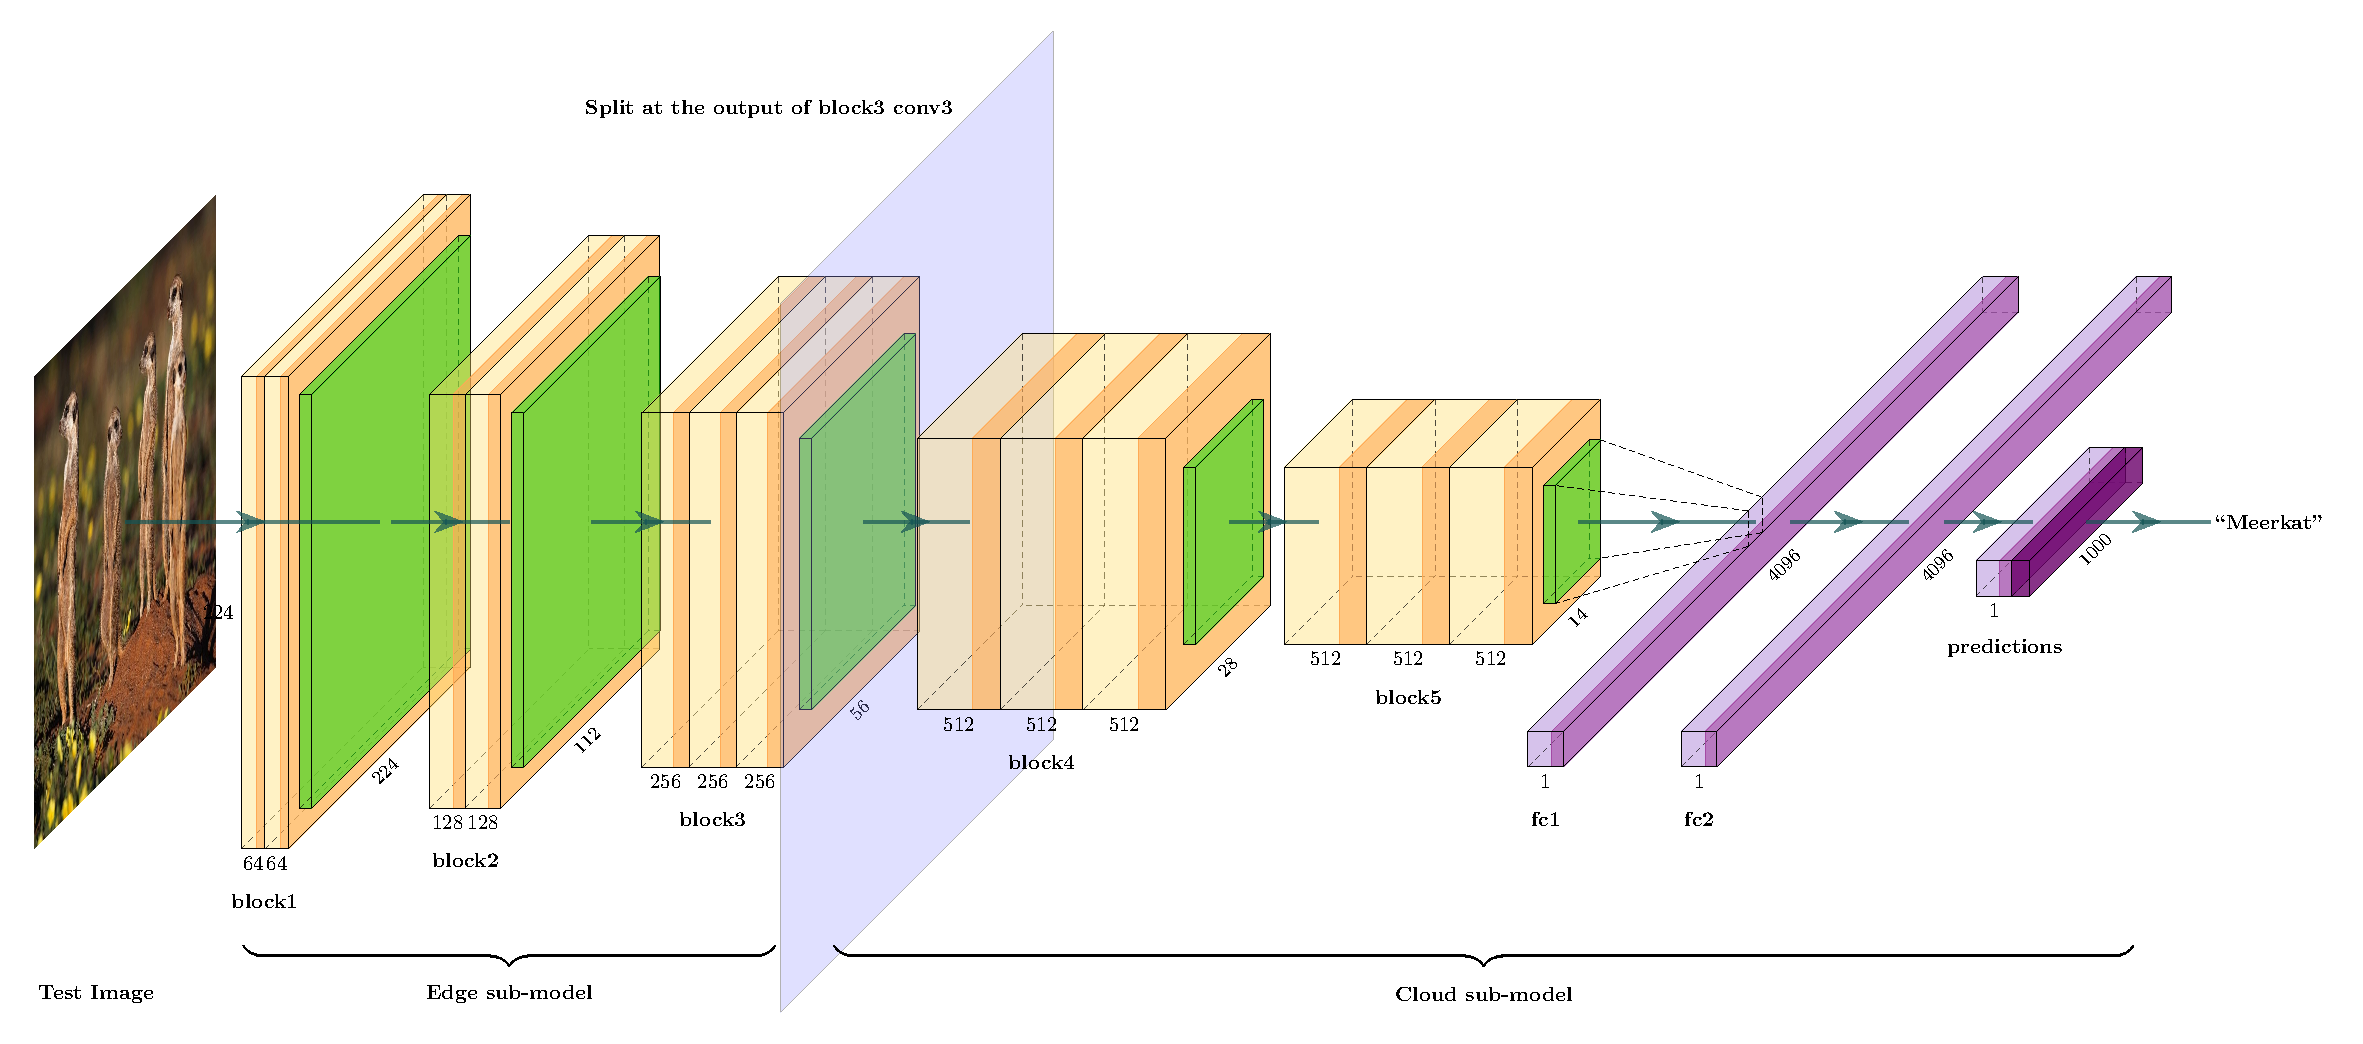
\includegraphics[scale = 0.27]{Figures/vgg16CI.pdf}
		\caption{Splitting a deep model into two sub-models: the mobile or device sub-model and the remote or cloud sub-model.}
		\label{fig:splitting}
	\end{figure}
\end{frame}

\section{DFTS}
\begin{frame}
	\frametitle{Deep Feature Transmission Simulator (DFTS)}
	\begin{itemize}
		\item DFTS was developed to simulate packet-based transmission of deep features over unreliable communication channels \footnote{\tiny{H. Unnibhavi, H. Choi, S. R. Alvar, and I. V. Bajić, “Dfts:
				Deep feature transmission simulator,” 2018.}} \cite{unnibhavi2018dfts}.
		\item DFTS simulations can include a Gilbert-Elliot channel, a random loss channel or a perfect channel (packets never incur any damage).
		\item $n$ bit quantization can be applied to deep feature packets before transmission.
		\item To conceal errors in damaged tensors, DFTS can do linear interpolation and nearest neighbor interpolation.
	\end{itemize}
\end{frame}

\begin{frame}
	\frametitle{Updating DFTS}
	\begin{itemize}
		\item DFTS was developed with TensorFlow 1.1.2 and Keras 2.2.2.
		\item Various changes in TensorFlow version 2 (discussed in the \textit{Effective Tensorflow 2} guide\footnote{\tiny{\url{https://www.tensorflow.org/guide/effective_tf2}}} \cite{tfv2}) break the operation of DFTS.
		\item It is possible to run DFTS version 1 in TensorFlow 2 by disabling the v2 behavior.
		\item A number of higher-level API calls in DFTS were modified to become TF 2 compatible. 
	\end{itemize}
\end{frame}

\begin{frame}
	\frametitle{Splitting a DNN into a mobile and a cloud client}
\end{frame}

\begin{frame}
	\frametitle{Packetization}
	\begin{itemize}
		\item 
	\end{itemize}
\end{frame}

\begin{frame}
	\frametitle{Channel model}
	\begin{itemize}
	\item The channel model aims to. Three possibilities: no channel, Gilbert-Elliott channel \& Random Loss channel.
	\item The Gilbert-Elliott model has been shown to fittingly capture real-time observed packet loss patterns over real-time services over the Internet \footnote{\tiny{G. Hasslinger and O. Hohlfeld, “The gilbert-elliott model for packet loss in real time services on the internet,” in 14th GI/ITG Conference - Measurement, Modelling and Evalutation of Computer and Communication Systems, pp. 1–15, 2008.}}. \cite{5755057}.
\end{itemize}
\end{frame}

\begin{frame}
	\frametitle{The Gilbert-Elliott channel model}
\begin{itemize}
	\item 8 rows per packet, so a $224 \times 224 \times 3$ tensor is packetized into 28 packets of $8 \times 224$ features per channel.
	\item Gilbert-Elliott channel of loss probability $P_B = 10\%$ and average burst length of $L_B = 4$ packets.
\end{itemize}
	\begin{figure}[H]
		\centering
		\begin{subfigure}{.25\linewidth}
			\centering
			
\includegraphics[width = \linewidth]{Figures/gridraftertrans.png}
			\caption{Channel \# 0.}
		\end{subfigure}%
		\hspace{1em}% Space between image A and B
		\begin{subfigure}{.25\linewidth}
			\centering
			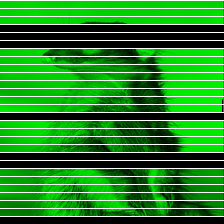
\includegraphics[width = \linewidth]{Figures/gridgaftertrans.png}
			\caption{Channel \# 1.}
		\end{subfigure}%
		\hspace{2em}% Space between image B and C
		\begin{subfigure}{.25\linewidth}
			\centering
			
\includegraphics[width = \linewidth]{Figures/gridbaftertrans.png}
			\caption{Channel \# 2}
		\end{subfigure}
		\caption{The RGB channels of an image packetized and transmitted through a Gilbert-Elliott channel.}
	\end{figure}
\end{frame}


\begin{frame}
	\frametitle{Running DFTS simulations}
	\begin{itemize}
		\item The \textit{BrokenModel} class imports Tensorflow, which is best run on GPU.
		\item The \textit{Channel} error concealment and tensor completion code are best run on CPU.
	\end{itemize}
\end{frame}



\section{Tensor Completion}
\begin{frame}
	\frametitle{Tensor Completion overview \& example}
\end{frame}

\begin{frame}
	\frametitle{How many iterations are sufficient?}
\end{frame}

\section{Error Concealment}
\begin{frame}
	\frametitle{Error Concealment overview}
\end{frame}


%------------------------------------------------
\section{Future work}
\begin{frame}
\frametitle{Recommendations for future work}

\begin{itemize}
	\item Public repo for DFTSv2: \url{https://github.com/AshivDhondea/DFTS_TF2}.
	\item The object detection task has yet to be implemented.
	\item Run ALTeC and other tensor completion methods in a DFTS experiment.
	\item Run tensor completion and error concealment methods with speed-matching.
\end{itemize}



\end{frame}
%--------------------------------------------------

%---------------------------------------------
\bibliographystyle{ieeetr}
\bibliography{Biblio/refs}
%----------------------------------------------------------------------------------------
\end{document} 
